\section{Função Logarítmica}
\begin{frame}
\frametitle{Definição} 
\begin{definicao}
A inversa da função exponencial de base $a$ é a \sub{função
logarítmica}
$$\log_a : \R_+^\ast \to \R,$$
que associa a cada número real positivo $x$ o número real $\log_a
x$, chamado \sub{logaritmo} de $x$ na base $a$. No caso de $a=10$,
escrevemos, por simplicidade, $\log_{10}x = \log
 x$.
\end{definicao}\pause
Pela definição de função inversa, tem-se
$$ a^{\log_a x}=x \ \ \ \text{ e } \ \ \ \log_a \paren{a^x} = x.$$
Assim, $\log_a x $ é o expoente ao qual se deve elevar a base $a$
para obter o número $x$. Ou seja,
$$ y = \log_a x \sse a^y = x.$$

\end{frame}


%------------------------------------------------------------------------------------------------------------
\begin{frame}
\frametitle{Propriedades} 

\begin{proposicao}
Seja $f: \R_+^\ast \to \R$ uma função logarítmica tal que $f(x) =
\log_a x$. Os seguintes valem para quaisquer  $x, y, b \in
\R_+^\ast$, $b \neq 1$ e qualquer $k \in \R$:
\begin{enumerate}[(a)]
	\item $\log_a \paren{xy} = \log_a x + \log_a y$;
	\item $\log_a x^k = k\cdot \log_a x$;
	\item $\log_a 1 = 0$;
	\item $\log_a x = \frac{\log_b x}{\log_b a}$;
	\item $f$ é bijetiva com contradomínio $\R$, logo é ilimitada superiormente e inferiormente;
	\item O gráfico de $f$ é traçado por uma linha contínua;
	\item $f$ é crescente se $a>1$ e decrescente se $0<a<1$.
\end{enumerate}
\end{proposicao}


\end{frame}

%------------------------------------------------------------------------------------------------------------
\begin{frame}
	\frametitle{Exemplos} 

	\begin{exemplo}
		Use as aproximações dos logaritmos abaixo para calcular $\log 300$, $\log 15{,}5$, $\log 225$ e $\log_{100}10$. Além disso, calcule o produto $17 \cdot 5$ utilizando somente a tabela abaixo e a operação de soma de números.
		\begin{center}
			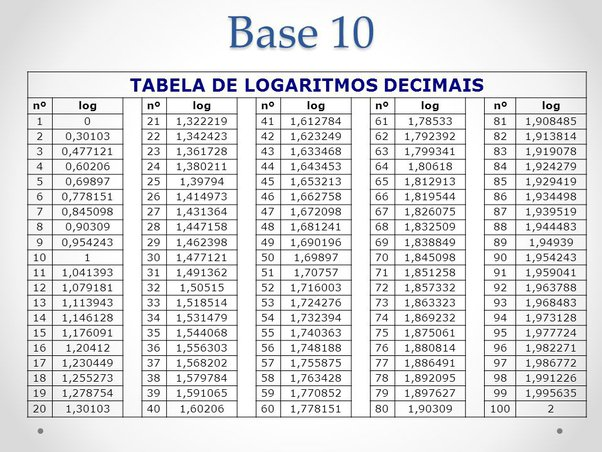
\includegraphics[width=7.1cm]{figures/tabua-log.jpg}
			\end{center}
		\end{exemplo}
	\end{frame}

%------------------------------------------------------------------------------------------------------------
\begin{frame}
	\frametitle{Exemplos} 

	\begin{exemplo}
	No Exemplo \ref{exem-alga} calculamos que, se uma alga que duplica sua área a cada dia cobre um determinado lago em 100 dias, então duas águas cobrirão o mesmo lago em 99 dias. Porém, ficou em aberto em quantos dias 3 algas cobrirão o mesmo lago. Além disso, defina uma função que calcula o número de dias que uma quantidade qualquer de algas cobre o lago.
	\end{exemplo}
	
	
	\end{frame}